\chapter{Sharing Immutable Data}
\label{chapter:sharing-immutable-data}

If you examine any Java
heap, you will find that a
large amount of the data is duplicated. At one extreme, 
there are often thousands of copies of the same boxed
integers, especially 0 and 1. At the other extreme, there may be many
 small data
structures that have the same shape and data. 
And, of course, duplicate strings are extremely common.
This chapter describes various
techniques for sharing read-only data to avoid
duplication, including a few low-level mechanisms that Java provides.
\autoref{sec:literals} looks at sharing literal data, known at compile time. 
The rest of the chapter describes techniques for sharing more
dynamic data.

\section{String Literals and \code{enum} Types}
\label{sec:literals}

Duplicate strings are not only one of the
most common sources of memory waste, they are also very expensive, since even
small strings incur a large overhead. Fortunately, it is not
hard to eliminate string duplication. 

 One technique is to represent strings as  
literals whenever possible. Duplication problems arise because dynamically
 created \class{Strings}
are stored in the heap without checking whether they already
exist. \class{String} literals, on the other hand, are stored in a
\emph{string constant pool} when classes
are loaded, where they are shared. Therefore, there is a big advantage to
\class{String} literals.

As an example, suppose an application
reads in property name-value pairs from files into tables:
\begin{shortlisting}
class ConfigurationProperties {
    ..
	void handleNextEntry() {
		String propertyName = getNextString();
		String propertyValue = getNextString();
		propertyMap.put(propertyName, propertyValue);
	}
}
\end{shortlisting}
The \class{Strings} stored in \code{propertyMap} are created dynamically. If 
there are just a few distinct property names in all of the input pairs, these
property names will be duplicated many times in the heap.

However, if you know in advance what all of the property names are, then you can
define them once as \class{String} literals, which can be shared among the
entries of \code{propertyMap}.
\begin{shortlisting}
class PropertyNames {
	final public static String numberOfUnits = ``NUM_UNITS'';
	final public static String minWidgets = ``MIN_WIDGETS'';
	..
}

class ConfigurationWithStaticProperties {
    void handleNextEntry() {
       String propertyName = getNextPropertyName(); 
       String propertyValue = getNextString();
       propertyMap.put(propertyName, propertyValue);
    }
}
\end{shortlisting}
The \code{getNextPropertyName} method reads in a property name, and returns
a pointer to a property name literal, stored in the JVM string
constant pool. Alternatively, defining an enumeration
type to encode property names may be a better stylistic choice.  Like
\class{String} literals, the \jre maintains just a single copy of each
\code{enum} constant.

A common
 mistake is to create a new \class{String}  from a \class{String} literal,
 which is usually completely unnecessary:
\begin{shortlisting}
class PropertyNames {
	final public static String numberOfUnits = 
	                           new String(``NUM_UNITS'');
	final public static String minWidgets = 
	                           new String(``MIN_WIDGETS'');
	..
}
\end{shortlisting}
Even though the standard library is smart enough to share
character arrays in this case, this code still creates redundant \class{String}
objects in the heap.

Using \class{String} literals to avoid duplication is only possible when the
\class{String} values are known in advance. 
\autoref{sec:sharing-pools} introduces the notion of a sharing pool for
sharing dynamic data. \autoref{sec:sharing-strings} describes the Java
string interning mechanism, which uses a built-in string sharing pool to
eliminate duplication.

\section{Sharing Pools}
\label{sec:sharing-pools}

Suppose an application generates a lot of duplicated data and the values
are unknown before execution. 
You can eliminate data duplication by using a \emph{sharing pool}, also known
as a \emph{canonicalizing map}. 
A sharing pool will eliminate not just duplicate data, 
but all of its associated overhead. Since many Java data structures employ 
delegation in their designs, sharing duplicate data can avoid
multiple levels of identical objects.

An example is shown in \autoref{fig:sharing-pool}. The example is from a
text processing system, which assigns a type to each word in a document.
Each type is identified by a \class{String} type name.
The complete set of word types is known only at run time, so an \code{enum}
type cannot be used.  In \autoref{fig:sharing-pool-a}, objects A and B
are words that have been classified as having the same type. 
\autoref{fig:sharing-pool-b} shows objects A and B sharing the type
structure, which is stored in a sharing pool. In this example, each use of a
shared structure saves three objects.

\begin{shortlisting}
public class WordInContext {
	private int  locationInDocument;
	private Type type;  // The word's role in the sentence
}

public class Type {
	final private String typeName;
}
\end{shortlisting}

[TODO: Redraw sharing pool figure, making it a concrete example.]

\begin{figure}
\centering
	\subfigure[]{\label{fig:sharing-pool-a}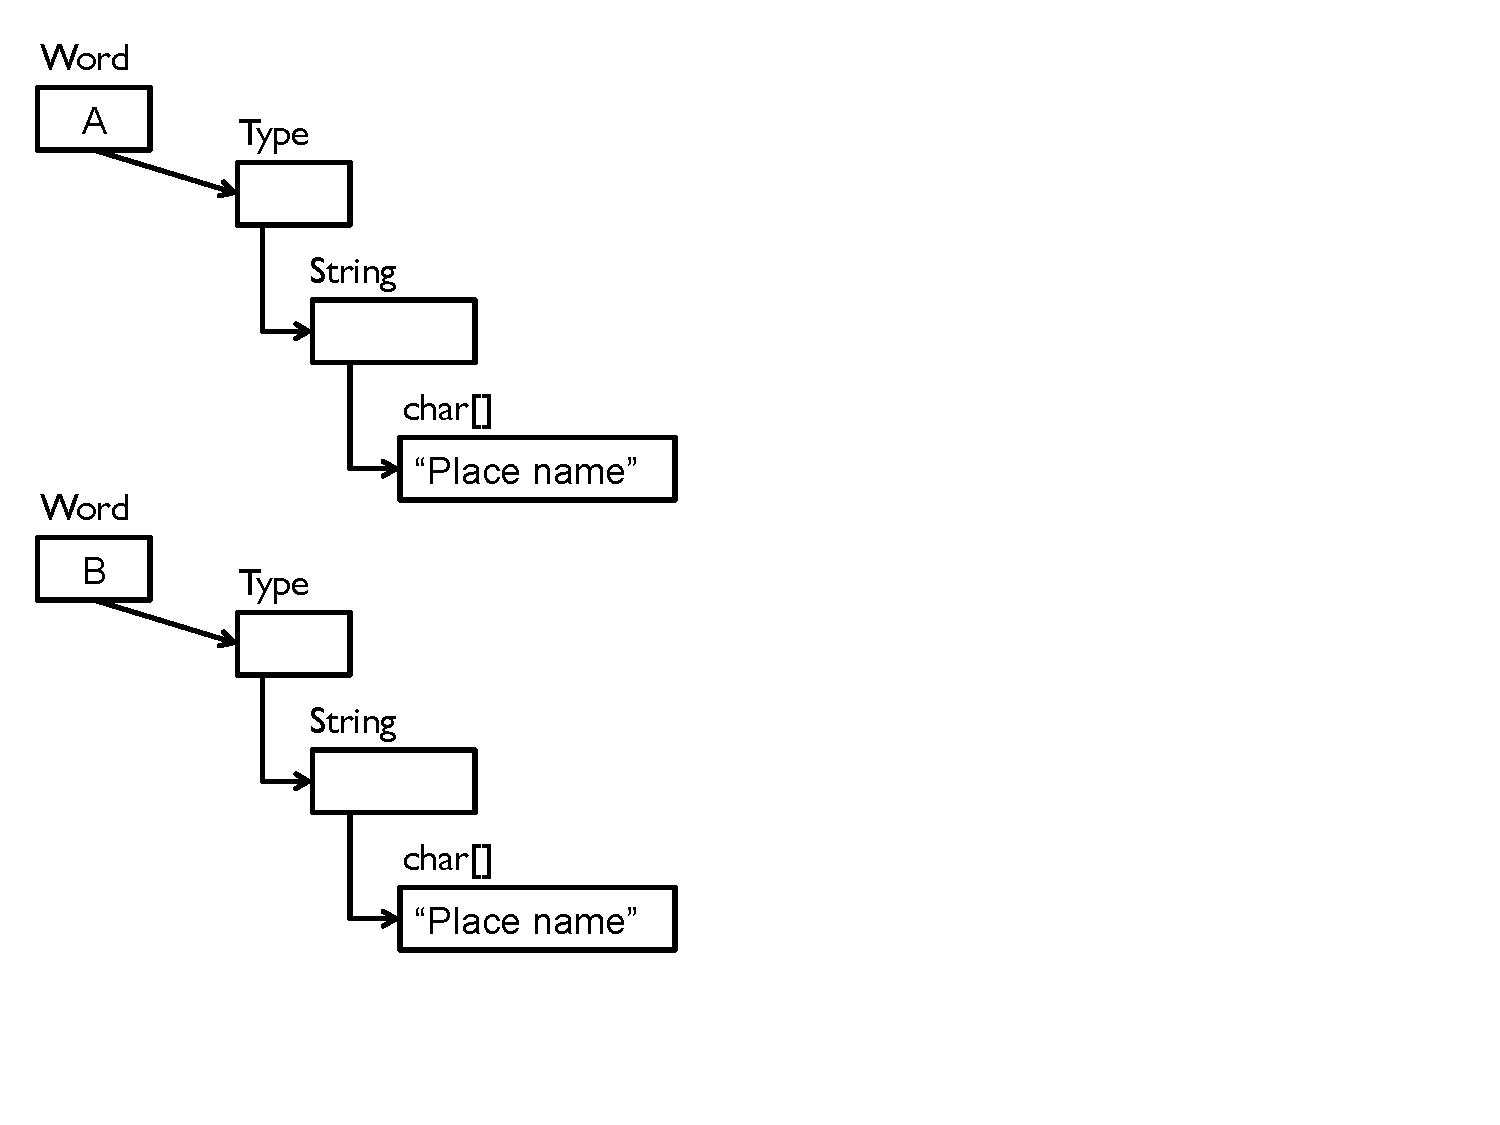
\includegraphics[width=0.3\textwidth]{part1/Figures/modelingdatatypes/sharing-pool-a.pdf}}
	\hspace{0.18\textwidth}
	\subfigure[]{\label{fig:sharing-pool-b}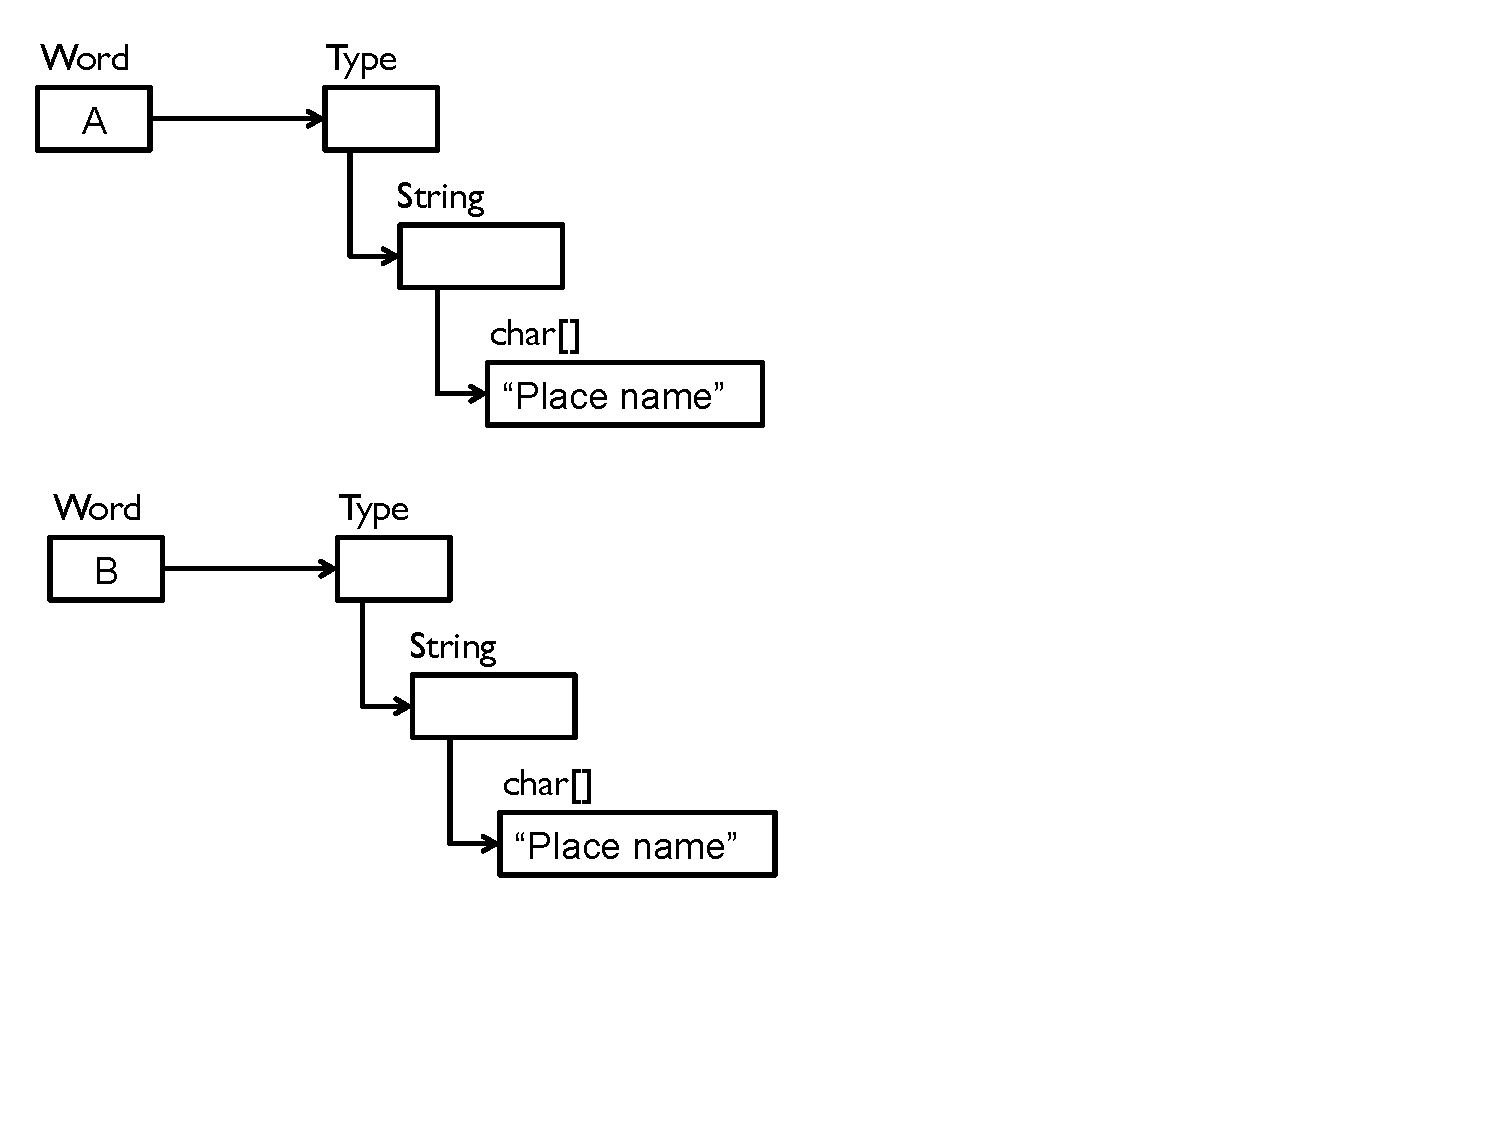
\includegraphics[width=0.445\textwidth]{part1/Figures/modelingdatatypes/sharing-pool-b.pdf}}
    \caption{(a) Words A and B point to duplicated data. (b) Words A and B
    share the same data, stored in a sharing pool.}
	\label{fig:sharing-pool}
\end{figure}

\callout{callout:sharing-pool}{Sharing Pool}{
A \emph{sharing pool} is a centralized structure
that stores canonical, read-only data that would otherwise be replicated in many
instances. A sharing pool itself is usually some sort of hash table, although it
could be implemented in other ways.
}

There are several issues that you need to be aware of before using a sharing
pool.
\paragraph{Shared objects must be immutable.} Changing shared data can
have unintended side effects. For example, 
changing the contents of the Type that A points to in
\autoref{fig:sharing-pool-b}, would also change the type of B.

\paragraph{The result of \code{equals} testing should be the same,
whether or not objects are shared.}
Always use \code{equals} to compare shared objects; never rely on \code{==}.
In \autoref{fig:sharing-pool},
\code{A.type == B.type} is false in \ref{fig:sharing-pool-a} and true in
\ref{fig:sharing-pool-b}, which can lead to very subtle bugs.
Some sharing pool implementations do not guarantee that all
duplicates will actually be shared. Avoiding \code{==} also allows
you to safely change your design, should you later decide to share a different set of instances, or to not share data at all.
\footnote{An argument sometimes heard for sharing data is that it will
allow for speedier comparisons, by letting the application use \code{==} rather
than \code{equals}. In fact, most
 \code{equals} methods already perform this optimization, making the performance virtually identical.}
 
\paragraph{Sharing pools should not be used if there is limited sharing.}
A sharing pool itself can add
memory costs, typically the cost of a map entry for each instance stored in the
sharing pool.
If there is not much sharing, then the memory saved from
eliminating duplicates isn't enough to compensate for the
extra cost, and memory will be wasted instead of saved.  In \autoref{sec:quantifying-sharing-savings} is
a sample analysis of when it's worth sharing Strings.

% NMM 20110614 i thought this was a good idea, but in Java, a reference will
% always be cheaper than an object, because of the header!
%\paragraph{The shared data items must be sufficiently large.} The size of the
%each pooled data item must be large, relative to the cost of a reference ---
%when using a pool, you still need to pay at least one reference cost for
%each use of the pooled items. 

\paragraph{Sharing pools can have performance costs.}
Sharing pools can sometimes add a performance cost when creating new instances
to be shared.  First, each new instance requires a lookup and possible
addition to the sharing pool. Second, in a multithreaded
environment, checking and adding to the sharing pool can introduce latency if the sharing pool is synchronized.
The use of shared instances, however, does not incur any extra
time costs.

\paragraph{Sharing pools should be either stable or garbage collected.} 
In Figure~\ref{fig:sharing-pool-b}, the sharing pool stores an object
that no other object is pointing to. Over time, the sharing pool can fill up with garbage, that is,
items that were once needed but not any more. If the
sharing pool is not purged of these unused items, there will be a
leak that will eventually use up more and more memory. 
However, if there are only a small number of shared instances,
or if the set of shared instances is unchanging for the lifetime of the pool,
then garbage collection need not to be a concern.

Fortunately, Java provides a few built-in mechanisms that take care of
these concerns for some common cases.

\section{Sharing Strings}
\label{sec:sharing-strings}
\index{Interning}

%Before storing a 
%To use a sharing pool, before storing a new
%\class{String}, first check the pool to see if it is already there. If it is,
%reuse it; otherwise, add the new string to the pool. 
%One catch is that if you end up adding many strings to
%the pool that are never reused, then you will waste memory, since the pool
%structure itself has overhead. So you need to have a good idea
%which strings are likely to have duplicate values.

Since \class{String} duplication is so common, Java provides a built-in
string pool for sharing \class{Strings}. To share a
\class{String}, you simply call the method \code{intern} on it, and everything
is taken care of automatically. \class{String} wrapper objects will be shared,
along with their underlying \class{char[]}s. Since
\class{Strings} are immutable, sharing is safe.
However, the rule about not using \code{==} still holds on shared
\class{Strings}.  Remember that only some
\class{Strings} will be shared in any application, namely those specific
instances that you choose to intern.

In the example from ~\autoref{sec:literals},
\class{ConfigurationWithStaticProperties} eliminates property
name duplication but not
property value duplication. Suppose you know that there are
not too many distinct values, but you don't know what they are. In this case,
property values are perfect candidates for interning.
\begin{shortlisting}
 
 class ConfigurationPropertiesWithInterning {
    void handleNextEntry() {
       PropertyName propertyName = getNextPropertyName(); 
       String propertyValue = getNextString().intern();
       propertyMap.put(propertyName, propertyValue);
    }
}
\end{shortlisting}

The call to \code{intern} adds the new property value \class{String}
 to the internal string
pool if it isn't there already, and return a pointer to it. Otherwise, the
new \class{String} is a duplicate, and a previously saved \class{String} is
returned.

Interned \class{Strings} are stored in a separate heap known as the
\emph{perm space}. There's a memory cost for each shared \class{String}, so
interning \class{Strings} indiscriminately will waste memory. 
Exceeding the size of the perm space will result in an exception:
\code{java.lang.OutOfMemoryError:PermGen space}
\footnote{This is an issue only for the \oracle \jre. The \ibm \jre places no
fixed limit on interned \code{Strings}.}. There are parameters to adjust
the perm space size. See \autoref{chapter:jre-options} for details. 
 Fortunately, the \jre performs garbage collection on the
internal string pool, so there is no danger of a memory leak.
\index{Permspace Heap}

The built-in interning mechanism is synchronized, and can incur a latency cost
in a multithreaded environment, when new \class{Strings} are interned.
The book Effective Java\cite{EffectiveJavaBook}, pp. xxx-yyy, gives an example
of how to build a concurrent sharing mechanism for \class{Strings}.

 %    * Literal strings within the same class in the same package represent
%     references to the same String object. * Literal strings within different
 %    classes in the same package represent references to the same String
%     object. * Literal strings within different classes in different packages
 %    likewise represent references to the same String object. * Strings
 %    computed by constant expressions are computed at compile time and then
   %  treated as if they were literals. * Strings computed by concatenation at
    % run time are newly created and therefore distinct.
\section{Sharing \class{Integers} and Other Boxed Scalars}

As of \javafive, the Java library provides sharing pools for
\class{Integers} and some of the other boxed scalars. These pools work
differently from string interning, where you first create a \class{String} and
then call its \code{intern} method.  To take advantage of \class{Integer}
sharing, simply call the factory method \code{Integer.valueOf(int i)}
whenever you want to create a new \code{Integer}. Unlike the string pool, the
integer pool is initialized to store all \class{Integers} in a fixed range, from
-128 to 127 by default. The factory method returns a
pointer to an \class{Integer} in the pool, provided \code{value} is in
range; otherwise it returns a new \class{Integer}. For example,
the code in \autoref{fig:integer-sharing-pool} stores \class{Integers} from 1 to
500 in an array.
\code{valueOf} returns an existing \class{Integer}
for the first 127 numbers, and, for the rest of the numbers, \code{valueOf}
returns a new \class{Integer} instance.

\begin{wrapfigure}{r}{0.4\textwidth}
\centering
\begin{framedlisting}
for (int i=1; i<=500; i++) {
 numbers[i] = Integer.valueOf(i);
}
\end{framedlisting}
\caption{By using the \code{valueOf} method, you can leverage the standard
library's integer sharing pool.}
\label{fig:integer-sharing-pool}
\end{wrapfigure}

Because the \class{Integer} sharing pool is pre-initialized and fixed in size,
it's usually a good idea to call \code{Integer.valueOf}, instead of
the constructor, whenever you need a new \class{Integer}. The pooling aspect is
very cheap, and you never have to worry about garbage collection, wasting memory, or concurrency issues.
You do have to be careful, however, to avoid using \code{==} to compare
\class{Integers}, since it's impossible to know with certainty which instances
are actually shared. As always, using \code{equals} is a better
practice.

[TODO: fix this to say it can only be increased  Move
specifics of AutoBoxCacheMax to Appendix] [TODO: mention autoboxing here or in
Appendix, along with JLS requirement].
There is a JVM parameter to
change the upper limit of the \class{Integer} sharing pool. By adding \code{-Djava.lang.Integer.IntegerCache.high=100} to your
application's command line, the pooled integers will range over the values -128
to 100.


The \jre provides a similar \code{valueOf} method for sharing each of the boxed
scalars. TODO: char and short In
some cases, such as \class{float}, there is no sharing actually implemented, at least as of \javasix. For \class{Boolean} and \class{Byte}, a
shared constant is returned for every possible value. In general, there is
no penalty for always using \code{valueOf}.

The exception to this rule is if you expect to have
boxed scalars such as \class{Integer}s with a large number of copies
of values lying outside the range of the built-in pool. In
this case you will not get the benefit of the built-in mechanism, and it
may be worth implementing your own sharing instead.  When sharing something
as small as a boxed scalar, however, there must be a very
high degree of duplication to make the extra overhead of your sharing mechanism worthwhile.

\section{Sharing Your Own Structures}
\label{sec:canonicalizing-maps}

Beyond strings and boxed scalars, there can be other kinds of
duplicated data structures that consume large portions of the heap. 
There is no built-in Java mechanism to share data
in general, so you have to implement a sharing pool for them from
scratch. All of the sharing pool issues from \autoref{sec:sharing-pools} need
to be addressed. The shared objects or structures must be immutable, they must not be
compared using \code{==}, there must be sufficient memory savings from sharing
to justify the sharing pool, and the sharing pool must not cause a memory leak. 

There are two common styles of implementing your own sharing pools, depending on
the complexity of the data being shared.  We illustrate both in this section. 
For the purposes of this discussion we assume that the set of shared data is
always needed throughout the run, so there is no need to worry about garbage collection. In
\autoref{sec:sharing-pools-safety} we revisit these two examples, and show how
to implement sharing pools with garbage collection.  We leave the addition of
concurrent access as an exercise. 

To illustrate one common style of user-written sharing pool, consider a graph
where the nodes have annotations, many of which are duplicates. Each annotation is a single
object, containing a few scalar fields, recording whether a node has been
visited, and the reason for the visit.  Both the graph and the annotations are modified
dynamically. Assume for now that the same universe of annotations is needed for
the duration of the run. The main requirement is the ability to find and
retrieve existing annotations quickly to share them.

\begin{wrapfigure}{r}{0.5\textwidth}
\centering
\begin{framedlisting}
HashMap<Annotation, Annotation> canonicalizingMap;
\end{framedlisting}
\end{wrapfigure}

Interestingly, none of the common collection classes meet this requirement
out of the box. A \class{HashSet} can store \class{Annotation}s uniquely, but
retrieving an existing \class{Annotation} is not easy. The \class{HashSet}
can let you know whether an equivalent item already
exists in the set, but can not return that item quickly. To get the
preexisting item, you would need to iterate over the entire set. The
most common approach is to use a
\class{HashMap} that maps the \class{Annotation} to itself, as shown on the
right. This design assumes that an \class{Annotation} can serve as its own key.
In other words, that the \code{hashcode} and \code{equals} methods are
defined on \class{Annotation} so that they ensure uniqueness. Note that, unless overridden, \code{equals} is
implemented as \code{==}, so sharing data structures typically requires writing
a new \code{equals} method.  

Callers must create an instance of \class{Annotation} in order
to find out whether it's already in the shared pool. This
is similar to the pattern of using \code{String.intern}, where you create a new
\code{String} in order to see if a matching shared \code{String} exists. Therefore, this type
of canonicalizing map only makes sense when sharing relatively simple data
that is inexpensive to create.

\begin{wrapfigure}{r}{0.5\textwidth}
\centering
\begin{framedlisting}
HashMap<String, Type> canonicalizingMap;
\end{framedlisting}
\end{wrapfigure}

Suppose now that we would like to share more complex data, such as the type
information from \autoref{fig:sharing-pool}. In this example, the type is
uniquely identified by a \class{String} type name. Each shared structure
consists of three objects. Rather than asking the programmer to create a new \class{Type} structure only to discover
that it exists in the pool, we can instead use the type name as the key, as
shown on the right. That way callers of the sharing pool only have to create a
\code{String} in order to find or retrieve the \class{Type}. In this example we save the creation of
one object for each new instance of the structure created.  For more complex structures the savings
are even more. 


%A common term for this structure is a \emph{canonicalizing map}.

\index{Canonicalizing Map}

\section{Quantifying the Savings}
\label{sec:quantifying-sharing-savings}

Before implementing a sharing scheme, we can estimate the
space savings, to make sure it's worth the effort, and to make there isn't a
net gain in memory usage.  Here is a sample analysis of sharing \class{Strings}.
This style of analysis can be applied to other types of shared data.

[TODO: Move just the string interning analysis from the chapter on
bulk storage.]

The techniques described in this chapter for sharing immutable
data can lead to substantial savings for many applications.  All of these
techniques are within the bounds of standard, object-oriented programming
practice. Later in the book, in \autoref{chapter:large-long-lived}, we look at
bulk storage and sharing techniques that stretch beyond the normal Java box in
order to achieve even greater space savings. 


%There is an important variant of a sharing pool called the Bulk Sharing
%Pool. Like a normal sharing pool, the goal of a bulk sharing pool is to
%amortize the memory costs of storing data. However, rather than mitigate the
%costs of data duplication, a bulk sharing pool aims to amortize the costs of
%Java object headers across the elements in a pool. This is a topic that
%stretches notions of how to store data beyond the normal Java box, and so will
%be discussed, along with many similar matters, in .


\section{Summary} 
Not only are Java heaps bloated from too much overhead, they
are also bloated from duplicated data. If you know that your application
generates many copies of the same data, then you should find a way to share the
data. Java provides several built-in sharing mechanisms:

\begin{itemize}
  \item you can use \class{String} literals or \code{enum} constants to share
  data that is known at compile time.
  \item The \jre maintains a sharing
  pool for \class{Strings}. Use \class{String} interning to make use of this
  sharing pool.
  \item The standard library maintains fixed-size pools for
   a fixed range of \class{Integers}, and other boxed scalars. You should use
   \code{valueOf} to create boxed scalars, instead of a constructor.
\end{itemize}

You can implement your own sharing pool using \class{Map} classes.

When sharing data, you should remember these four rules:
\begin{itemize}
  \item Shared objects must be immutable.
  \item The result of \code{equals()} testing should be the same, whether or
not objects are shared.  Always use \code{equals()} rather than \code{==} to
test equality.
  \item Sharing pools should not be used if there is limited sharing.
  \item Unless the set of shared objects is small or is stable for
  the lifetime of the sharing pool, shared objects must be garbage
  collected.
\end{itemize}





